% !TeX program = xelatex
% !TeX encoding = utf-8
\documentclass[aspectratio=169, 11pt]{beamer}

% ==============================================================================
% Cấu hình font và ngôn ngữ
% ==============================================================================
\usepackage{fontspec}
\defaultfontfeatures{Ligatures=TeX}
\setsansfont{Segoe UI}[
  BoldFont = {Segoe UI Bold},
  ItalicFont = {Segoe UI Italic},
  BoldItalicFont = {Segoe UI Bold Italic}
]
\setmonofont[Scale=0.90]{Consolas}[
  BoldFont = {Consolas Bold},
  ItalicFont = {Consolas Italic},
  BoldItalicFont = {Consolas Bold Italic}
]

\usepackage{amsmath,amssymb}
\usepackage{booktabs}
\usepackage{array}
\usepackage{graphicx}
\usepackage{xcolor}
\usepackage{fancyvrb}
\usepackage[many]{tcolorbox}
\usepackage{tikz}
\usetikzlibrary{arrows.meta, positioning, calc, patterns, shapes.geometric}

\graphicspath{{../assets/images/}{../assets/images/figures/}{./}{figures/}}

% ==============================================================================
% Bảng màu giao diện
% ==============================================================================
\definecolor{DarkMain}{RGB}{20, 20, 20}       % Màu chủ đạo
\definecolor{BoxMain}{RGB}{222, 225, 230}    % Màu khối chính
\definecolor{BoxDeep}{RGB}{185, 189, 196}    % Màu gợn sóng
\definecolor{BoxSub}{RGB}{246, 247, 249}     % Màu khối phụ
\definecolor{DisabledBg}{RGB}{236, 237, 240} % Màu trạng thái vô hiệu hóa
\definecolor{CodeBg}{RGB}{247, 248, 250}     % Màu nền khối mã nguồn
\definecolor{TextDark}{RGB}{20, 20, 20}      % Màu chữ chính
\definecolor{TextMuted}{RGB}{100, 102, 108}  % Màu chữ chú thích

% ==============================================================================
% Cấu hình giao diện Beamer
% ==============================================================================
\useinnertheme{default}
\useoutertheme{default}
\setbeamertemplate{navigation symbols}{}
\setbeamersize{text margin left=0.95cm, text margin right=0.95cm}

\setbeamercolor{background canvas}{bg=white}
\setbeamercolor{normal text}{fg=TextDark}
\setbeamercolor{frametitle}{fg=DarkMain, bg=white}
\setbeamercolor{itemize item}{fg=DarkMain}
\setbeamercolor{itemize subitem}{fg=DarkMain}
\setbeamercolor{enumerate item}{fg=DarkMain}

% Định dạng danh sách
\setbeamertemplate{itemize item}{\textbf{\color{DarkMain}--}}
\setbeamertemplate{itemize subitem}{\textbf{\color{TextMuted}--}}
\setbeamertemplate{enumerate item}{\textbf{\color{DarkMain}\insertenumlabel.}}

% Định dạng tiêu đề slide
\setbeamertemplate{frametitle}{
  \vspace{0.30cm}
  \noindent{\fontsize{18pt}{22pt}\selectfont\bfseries\color{DarkMain}\insertframetitle}\par
  \vspace{0.14cm}
  \noindent{\color{DarkMain}\rule{\textwidth}{1.05pt}}\par
  \vspace{0.06cm}
}

% Định dạng chân trang
\newcommand{\currentsectionname}{}
\newcommand{\setsectionfooter}[1]{\renewcommand{\currentsectionname}{#1}}

\setbeamertemplate{footline}{
  \hbox to \paperwidth{%
    \hspace*{0.95cm}%
    {\fontsize{8.2pt}{10pt}\selectfont\color{TextMuted}%
      Sự kiện và tương tác%
      \ifx\currentsectionname\empty\else\ \textbar\ \currentsectionname\fi
    }%
    \hfill
    {\fontsize{8.5pt}{10pt}\selectfont\bfseries\color{DarkMain}\insertframenumber\,/\,\inserttotalframenumber}%
    \hspace*{0.95cm}%
  }%
  \vspace*{0.26cm}%
}

% ==============================================================================
% Định dạng khối mã nguồn
% ==============================================================================
\newcommand{\code}[1]{\leavevmode{\ttfamily\color{DarkMain}#1}}
\newcommand{\cmt}[1]{\leavevmode{\itshape\color{TextMuted}#1}}

\newtcolorbox{codepanel}{
  enhanced,
  frame hidden,
  borderline west={2.3pt}{0pt}{DarkMain},
  colback=CodeBg,
  sharp corners,
  halign=left,
  left=8pt,
  right=8pt,
  top=4.5pt,
  bottom=4.5pt,
  boxsep=0pt,
  before skip=2pt,
  after skip=2pt
}

% Cấu hình sơ đồ TikZ
\tikzset{
  >=Stealth,
  diagbox/.style={
    rectangle,
    rounded corners=2.2pt,
    draw=DarkMain,
    line width=0.9pt,
    fill=BoxMain,
    minimum height=0.92cm,
    align=center,
    font=\small\bfseries,
    text=TextDark
  },
  subbox/.style={
    rectangle,
    rounded corners=2.2pt,
    draw=DarkMain,
    line width=0.9pt,
    fill=BoxSub,
    minimum height=0.92cm,
    align=center,
    font=\small,
    text=TextDark
  },
  ghostbox/.style={
    rectangle,
    rounded corners=2.2pt,
    draw=TextMuted,
    dashed,
    line width=0.8pt,
    fill=white,
    minimum height=0.92cm,
    align=center,
    font=\small,
    text=TextMuted
  },
  flowarrow/.style={
    -{Stealth[length=2.3mm, width=1.7mm]},
    draw=DarkMain,
    line width=0.95pt
  },
  dasharrow/.style={
    -{Stealth[length=2.3mm, width=1.7mm]},
    draw=DarkMain,
    dashed,
    line width=0.9pt
  }
}

\begin{document}
\gdef\inserttotalframenumber{23}

% ==============================================================================
% Slide 1: Trang bìa
% ==============================================================================
\begin{frame}[plain]
  \vspace{0.2cm}
  \begin{columns}[c, onlytextwidth]
    \begin{column}{0.13\textwidth}
      \centering
      
\includegraphics[height=1.50cm]{figures/logo_truong.png}
    \end{column}
    \begin{column}{0.72\textwidth}
      \centering
      {\normalsize \textbf{TRƯỜNG ĐẠI HỌC BÁCH KHOA}}\\[0.05cm]
      {\normalsize \textbf{ĐẠI HỌC ĐÀ NẴNG}}\\[0.10cm]
      {\normalsize \textbf{KHOA ĐIỆN TỬ VÀ TRÍ TUỆ NHÂN TẠO}}
    \end{column}
    \begin{column}{0.13\textwidth}
      \centering
      
\includegraphics[height=1.55cm]{figures/logo_khoa.jpg}
    \end{column}
  \end{columns}

  \vspace{0.35cm}
  \begin{center}
    {\normalsize \textit{Báo cáo Tuần 13 --- Học phần: Lập trình Đa nền tảng}}
  \end{center}

  \vspace{0.25cm}
  \begin{center}
    {\LARGE \textbf{Chủ đề 7: Sự kiện và tương tác người dùng trong giao diện}}
  \end{center}

  \vspace{0.35cm}
  \begin{center}
    \begin{tabular}{rl}
      \textbf{Giảng viên hướng dẫn:} & TS. Nguyễn Duy Nhật Viễn \\[0.12cm]
      \textbf{Sinh viên thực hiện:}   & Lê Anh Khoa --- MSSV: 106230016 \\
                                     & Ngô Quang Thế --- MSSV: 106230028 \\[0.12cm]
      \textbf{Lớp sinh hoạt:}        & 23KTMT1
    \end{tabular}
  \end{center}

  \vfill
  \begin{center}
    {\footnotesize \color{TextMuted} Đà Nẵng, 2026}
  \end{center}
  \vspace{0.15cm}
\end{frame}

% ==============================================================================
% Slide 2: Mục tiêu và nội dung
% ==============================================================================
\setsectionfooter{}
\begin{frame}{Mục tiêu và nội dung}
  \vspace{0.32cm}
  \begin{columns}[T, onlytextwidth]
    \begin{column}{0.48\textwidth}
      {\large\bfseries Mục tiêu}\\[0.30cm]
      \begin{itemize}\setlength{\itemsep}{0.36cm}
        \item Nắm vững cơ chế \textbf{Callback}, thuộc tính \code{onPressed}, \code{onTap} và widget xử lý cử chỉ
        \item Phân biệt bản chất \textbf{sự kiện tương tác} và nơi lưu trữ \textbf{trạng thái}
        \item Cập nhật giao diện thông qua \code{setState()} và xây dựng phản hồi tương tác
      \end{itemize}
    \end{column}
    \hfill
    \begin{column}{0.47\textwidth}
      {\large\bfseries Nội dung}\\[0.30cm]
      \begin{enumerate}\setlength{\itemsep}{0.34cm}
        \item Tiếp nhận sự kiện và cử chỉ:\\[2pt]
              {\small \code{Callback}, \code{onPressed}, \code{onTap}, \code{GestureDetector}, \code{InkWell}}
        \item Sự kiện, trạng thái và \code{setState()}
        \item Phản hồi giao diện khi thao tác
        \item Thực nghiệm: Bảng điều khiển thiết bị
      \end{enumerate}
    \end{column}
  \end{columns}
\end{frame}

% ==============================================================================
% Slide 3: Phân công công việc
% ==============================================================================
\begin{frame}{Phân công công việc}
  \vspace{0.35cm}
  \renewcommand{\arraystretch}{1.55}
  \setlength{\tabcolsep}{6.5pt}
  \begin{tabular}{@{} l >{\raggedright\arraybackslash}p{2.85cm} >{\raggedright\arraybackslash}p{5.85cm} l l @{}}
    \toprule[0.9pt]
    {\bfseries\color{DarkMain}STT} &
    \multicolumn{1}{l}{{\bfseries\color{DarkMain}Họ và tên}} &
    \multicolumn{1}{l}{{\bfseries\color{DarkMain}Nội dung đảm nhiệm}} &
    {\bfseries\color{DarkMain}Slide} &
    {\bfseries\color{DarkMain}Đóng góp} \\
    \midrule[0.5pt]
    01 & Ngô Quang Thế\newline{\footnotesize\color{TextMuted}106230028} &
    Nghiên cứu \code{Callback}, \code{onPressed}, \code{onTap}, \code{GestureDetector}, \code{InkWell}; lập trình thẻ Đèn và Quạt &
    1--12 & 50\% \\[0.18cm]
    02 & Lê Anh Khoa\newline{\footnotesize\color{TextMuted}106230016} &
    Nghiên cứu \code{State}, cơ chế \code{setState()}, phản hồi UI; lập trình thẻ Máy bơm và Demo thực nghiệm &
    13--23 & 50\% \\
    \bottomrule[0.9pt]
  \end{tabular}

\end{frame}

% ==============================================================================
% PHẦN 1: TIẾP NHẬN SỰ KIỆN VÀ CỬ CHỈ
% ==============================================================================
\setsectionfooter{Tiếp nhận sự kiện và cử chỉ}

% ------------------------------------------------------------------------------
% Slide 4: Chu trình tương tác
% ------------------------------------------------------------------------------
\begin{frame}{Chu trình tương tác trong Flutter}
  \vspace{0.22cm}
  \begin{columns}[c, onlytextwidth]
    \begin{column}{0.43\textwidth}
      \centering
      \begin{tikzpicture}
        \node[diagbox, minimum width=3.5cm] (user) at (0, 2.2) {Widget tương tác};
        \node[subbox, minimum width=3.5cm]  (cb)   at (0, 0.65) {\textbf{Callback} \& \code{setState}};
        \node[subbox, minimum width=3.5cm]  (ui)   at (0, -0.9) {Giao diện mới (\code{build})};

        \draw[flowarrow] (user.south) -- (cb.north)
          node[midway, left=4pt, font=\small] {(1)};
        \draw[flowarrow] (cb.south) -- (ui.north)
          node[midway, left=4pt, font=\small] {(2)};
        \draw[dasharrow] (ui.east) .. controls +(1.30, 0.3) and +(1.30, -0.3) .. (user.east)
          node[midway, right=4pt, font=\small] {(3)};
      \end{tikzpicture}
    \end{column}
    \hfill
    \begin{column}{0.54\textwidth}
      \renewcommand{\arraystretch}{1.15}
      \setlength{\tabcolsep}{6pt}
      \begin{tabular}{@{} l >{\raggedright\arraybackslash}p{6.5cm} @{}}
        {\bfseries\color{DarkMain}(1)} & \textbf{Sự kiện kích hoạt Callback}\newline
        {\color{TextMuted}người dùng thao tác, widget gọi hàm xử lý} \\[0.42cm]
        {\bfseries\color{DarkMain}(2)} & \textbf{Cập nhật dữ liệu State}\newline
        {\color{TextMuted}thay đổi biến trạng thái thông qua \code{setState()}} \\[0.42cm]
        {\bfseries\color{DarkMain}(3)} & \textbf{Vẽ lại giao diện (Rebuild)}\newline
        {\color{TextMuted}hiển thị giao diện mới theo công thức \textbf{UI = f(State)}}
      \end{tabular}
    \end{column}
  \end{columns}
\end{frame}

% ------------------------------------------------------------------------------
% Slide 5: Callback
% ------------------------------------------------------------------------------
\begin{frame}[fragile]{Callback là gì?}
  \vspace{0.18cm}
  \begin{columns}[c, onlytextwidth]
    \begin{column}{0.47\textwidth}
      \centering
      \begin{tikzpicture}
        \node[diagbox, minimum width=2.45cm, minimum height=1.08cm] (btn) at (0, 0)
          {ElevatedButton\\[-1pt]{\scriptsize\normalfont\color{TextDark}\texttt{onPressed}}};
        \node[subbox, minimum width=2.35cm, minimum height=1.08cm] (fn) at (4.05, 0)
          {\texttt{batDen()}\\[-1pt]{\scriptsize\normalfont\color{TextMuted}hàm xử lý}};
        \draw[flowarrow] (btn.east) -- (fn.west)
          node[midway, above=3pt, font=\scriptsize\color{TextMuted}] {khi bấm};
      \end{tikzpicture}
    \end{column}
    \hfill
    \begin{column}{0.50\textwidth}
      \begin{codepanel}
\begin{Verbatim}[commandchars=§«»,fontsize=\fontsize{8.5pt}{12.5pt}\selectfont]
void batDen() { ... }

ElevatedButton(
  onPressed: batDen, §cmt«// Truyền tham chiếu»
  child: Text('Bật đèn'),
)
\end{Verbatim}
      \end{codepanel}
    \end{column}
  \end{columns}

  \vspace{0.44cm}
  \begin{itemize}\setlength{\itemsep}{0.25cm}
    \item Trong Dart, hàm là \textbf{đối tượng hạng nhất} (first-class object), có thể truyền làm tham số
    \item \code{Callback}: hàm giao cho widget để \textbf{tự gọi lại} khi sự kiện xảy ra
    \item Tách biệt phần \textbf{hiển thị giao diện} với phần \textbf{xử lý logic}
  \end{itemize}
\end{frame}

% ------------------------------------------------------------------------------
% Slide 6: Thuộc tính onPressed
% ------------------------------------------------------------------------------
\begin{frame}[fragile]{Thuộc tính onPressed}
  \vspace{0.16cm}
  \begin{columns}[c, onlytextwidth]
    \begin{column}{0.42\textwidth}
      {\footnotesize\texttt{onPressed: batDen} (Kích hoạt)}\\[0.1cm]
      \begin{tikzpicture}
        \node[diagbox, rounded corners=3pt, minimum width=4.3cm, minimum height=0.80cm]
          {Bật tất cả};
      \end{tikzpicture}

      \vspace{0.28cm}
      {\footnotesize\texttt{onPressed: null} (Vô hiệu hóa)}\\[0.1cm]
      \begin{tikzpicture}
        \node[ghostbox, rounded corners=3pt, fill=DisabledBg, minimum width=4.3cm, minimum height=0.80cm]
          {Tắt tất cả};
      \end{tikzpicture}
    \end{column}
    \hfill
    \begin{column}{0.55\textwidth}
      \begin{codepanel}
\begin{Verbatim}[commandchars=§«»,fontsize=\fontsize{8.1pt}{12.2pt}\selectfont]
onPressed: batDen,       §cmt«// Tham chiếu hàm»
onPressed: () => bat(1), §cmt«// Hàm ẩn danh (lambda)»
onPressed: null,         §cmt«// Khóa nút (disabled)»

§cmt«// Sai: tự chạy ngay khi dựng UI»
§cmt«// onPressed: batDen(),»
\end{Verbatim}
      \end{codepanel}
    \end{column}
  \end{columns}

  \vspace{0.40cm}
  \begin{itemize}\setlength{\itemsep}{0.22cm}
    \item Nhận kiểu \code{VoidCallback?} (\code{void Function()?}); khi gán \code{null} nút sẽ tự động bị vô hiệu hóa (disabled)
    \item Không gọi trực tiếp \code{batDen()}, trừ khi bọc trong hàm ẩn danh \code{() => bat(1)}
  \end{itemize}
\end{frame}

% ------------------------------------------------------------------------------
% Slide 7: Thuộc tính onTap và chu trình chạm
% ------------------------------------------------------------------------------
\begin{frame}{Thuộc tính onTap và chu trình chạm}
  \vspace{0.24cm}
  \centering
  \begin{tikzpicture}
    % Nhánh 1: Chạm hợp lệ
    \node[anchor=west, font=\footnotesize\bfseries\color{DarkMain}] at (-6.50, 1.50) {Chạm hợp lệ};
    \node[subbox, minimum width=3.05cm, minimum height=0.82cm]  (d1) at (-4.98, 0.80) {\texttt{onTapDown}\\{\scriptsize\color{TextMuted}chạm xuống}};
    \node[subbox, minimum width=4.35cm, minimum height=0.82cm]  (u1) at (-0.40, 0.80) {\texttt{onTapUp}\\{\scriptsize nhấc tay trong vùng}};
    \node[diagbox, minimum width=3.05cm, minimum height=0.82cm] (t1) at (4.18, 0.80)  {\texttt{onTap}\\{\scriptsize\normalfont kích hoạt lệnh}};
    \draw[flowarrow] (d1) -- (u1);
    \draw[flowarrow] (u1) -- (t1);

    % Nhánh 2: Hủy chạm
    \node[anchor=west, font=\footnotesize\bfseries\color{TextMuted}] at (-6.50, -0.35) {Trượt ra ngoài};
    \node[subbox, minimum width=3.05cm, minimum height=0.82cm]   (d2) at (-4.98, -1.05) {\texttt{onTapDown}\\{\scriptsize\color{TextMuted}chạm xuống}};
    \node[subbox, minimum width=4.35cm, minimum height=0.82cm]   (u2) at (-0.40, -1.05) {Trượt tay ra ngoài vùng nút};
    \node[ghostbox, minimum width=3.05cm, minimum height=0.82cm] (t2) at (4.18, -1.05)  {\texttt{onTapCancel}\\{\scriptsize hủy thao tác}};
    \draw[flowarrow] (d2) -- (u2);
    \draw[dasharrow] (u2) -- (t2);
  \end{tikzpicture}

  \vspace{0.34cm}
  \begin{itemize}\setlength{\itemsep}{0.18cm}
    \item \textbf{Chạm hợp lệ}: \code{onTapDown} (chạm) $\to$ \code{onTapUp} (nhấc tay trong vùng) $\to$ kích hoạt lệnh \textbf{\code{onTap}}
    \item \textbf{Hủy thao tác}: trượt tay ra ngoài vùng widget kích hoạt \textbf{\code{onTapCancel}} (cho phép đổi ý khi chạm nhầm)
  \end{itemize}
\end{frame}

% ------------------------------------------------------------------------------
% Slide 8: GestureDetector
% ------------------------------------------------------------------------------
\begin{frame}[fragile]{GestureDetector: Bắt đa dạng cử chỉ}
  \vspace{0.18cm}
  \begin{columns}[c, onlytextwidth]
    \begin{column}{0.44\textwidth}
      \centering
      \begin{tikzpicture}
        \draw[draw=DarkMain, dashed, line width=0.9pt] (-2.6, -1.30) rectangle (2.6, 1.30);
        \node[anchor=south west, font=\footnotesize\ttfamily\color{DarkMain}] at (-2.6, 1.33) {GestureDetector (bọc ngoài)};
        \node[diagbox, minimum width=3.2cm, minimum height=1.05cm] at (0, 0.15) {Widget con bất kỳ};
        \node[font=\scriptsize\color{TextMuted}] at (0, -0.82) {\texttt{tap} \textbullet\ \texttt{doubleTap} \textbullet\ \texttt{longPress} \textbullet\ \texttt{pan}};
      \end{tikzpicture}
    \end{column}
    \hfill
    \begin{column}{0.53\textwidth}
      \begin{codepanel}
\begin{Verbatim}[commandchars=§«»,fontsize=\fontsize{8.5pt}{12.3pt}\selectfont]
GestureDetector(
  onTap: batTatQuat,
  onDoubleTap: doiTocDo,
  onLongPress: veCap1,
  child: FanCard(),
)
\end{Verbatim}
      \end{codepanel}
    \end{column}
  \end{columns}

  \vspace{0.38cm}
  \begin{itemize}\setlength{\itemsep}{0.22cm}
    \item Bọc ngoài \textbf{mọi widget} (\code{Container}, \code{Image}, thẻ tự thiết kế)
    \item Hỗ trợ đa dạng cử chỉ: chạm đơn, chạm đúp, nhấn giữ, kéo rê, thu phóng
    \item \textbf{Không có hiệu ứng hiển thị mặc định} khi người dùng chạm vào
  \end{itemize}
\end{frame}

% ------------------------------------------------------------------------------
% Slide 9: InkWell
% ------------------------------------------------------------------------------
\begin{frame}[fragile]{InkWell: Bắt tương tác chạm với hiệu ứng gợn sóng}
  \vspace{0.06cm}
  \begin{columns}[c, onlytextwidth]
    \begin{column}{0.44\textwidth}
      \centering
      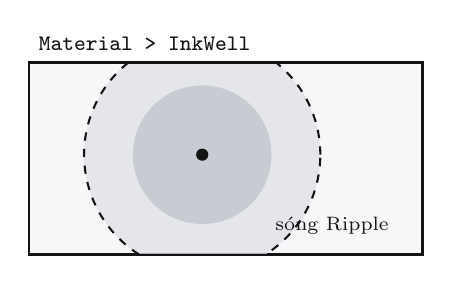
\begin{tikzpicture}
        \draw[draw=DarkMain, line width=0.95pt, fill=BoxSub] (-2.5, -1.22) rectangle (2.5, 1.22);
        \node[anchor=south west, font=\footnotesize\ttfamily\color{DarkMain}] at (-2.5, 1.25) {Material > InkWell};
        \begin{scope}
          \clip (-2.48, -1.20) rectangle (2.48, 1.20);
          \fill[BoxMain, opacity=0.75] (-0.3, 0.05) circle (1.50cm);
          \draw[DarkMain, dashed, line width=0.75pt] (-0.3, 0.05) circle (1.50cm);
          \fill[BoxDeep, opacity=0.65] (-0.3, 0.05) circle (0.88cm);
          \fill[DarkMain] (-0.3, 0.05) circle (2.2pt);
        \end{scope}
        \node[font=\scriptsize\color{TextDark}] at (1.35, -0.85) {sóng Ripple};
      \end{tikzpicture}
    \end{column}
    \hfill
    \begin{column}{0.53\textwidth}
      \begin{codepanel}
\begin{Verbatim}[commandchars=§«»,fontsize=\fontsize{8.3pt}{12.0pt}\selectfont]
Material(
  color: Colors.transparent,
  child: InkWell(
    borderRadius: BorderRadius.circular(16),
    onTap: batTatDen,
    child: LampCard(),
  ),
)
\end{Verbatim}
      \end{codepanel}
    \end{column}
  \end{columns}

  \vspace{0.36cm}
  \begin{itemize}\setlength{\itemsep}{0.22cm}
    \item Tạo hiệu ứng \textbf{gợn sóng} (Material Ripple) lan tỏa từ điểm chạm
    \item Cần có widget tổ tiên kiểu \code{Material} để vẽ hiệu ứng sóng (thiếu thì vẫn nhận chạm nhưng không hiện sóng gợn)
  \end{itemize}
\end{frame}

% ------------------------------------------------------------------------------
% Slide 10: So sánh InkWell và GestureDetector
% ------------------------------------------------------------------------------
\begin{frame}{So sánh InkWell và GestureDetector}
  \vspace{0.15cm}
  \renewcommand{\arraystretch}{1.30}
  \setlength{\tabcolsep}{8pt}
  \centering
  \begin{tabular}{@{} l >{\raggedright\arraybackslash}p{4.25cm} >{\raggedright\arraybackslash}p{4.55cm} @{}}
    \toprule[0.9pt]
    & \multicolumn{1}{l}{{\bfseries\color{DarkMain}InkWell}} & \multicolumn{1}{l}{{\bfseries\color{DarkMain}GestureDetector}} \\
    \midrule[0.5pt]
    \textbf{Hiệu ứng chạm}        & Gợn sóng (Material Ripple) & Không có (vô hình) \\
    \textbf{Ràng buộc Widget cha} & Cần \code{Material} tổ tiên & Bọc trực tiếp mọi widget \\
    \textbf{Cử chỉ hỗ trợ}        & Chạm cơ bản (\code{tap}, \code{longPress}) & Đa cử chỉ (kéo, vuốt, thu phóng) \\
    \textbf{Dùng khi}             & Thẻ, danh sách cần phản hồi chạm & Vùng tương tác riêng, đa cử chỉ \\
    \bottomrule[0.9pt]
  \end{tabular}

  \vspace{0.22cm}
  \centering
  {\small\color{TextMuted} Lưu ý: Đối với thao tác nhấn thông thường, nên ưu tiên dùng widget nút bấm có sẵn (\code{ElevatedButton}, \code{FilledButton}, \code{IconButton})}
\end{frame}

% ==============================================================================
% PHẦN 2: TRẠNG THÁI VÀ CẬP NHẬT UI
% ==============================================================================
\setsectionfooter{Trạng thái và cập nhật UI}

% ------------------------------------------------------------------------------
% Slide 11: Phân biệt sự kiện và trạng thái
% ------------------------------------------------------------------------------
\begin{frame}{Phân biệt sự kiện và trạng thái}
  \vspace{0.18cm}
  \begin{columns}[T, onlytextwidth]
    \begin{column}{0.47\textwidth}
      \begin{tikzpicture}
        \node[subbox, dashed, minimum width=6.4cm, minimum height=0.80cm] {\textbf{Sự kiện (\texttt{Event})} -- Tức thời};
      \end{tikzpicture}
      \vspace{0.16cm}
      \begin{itemize}\setlength{\itemsep}{0.22cm}
        \item Xảy ra trong khoảnh khắc người dùng thao tác
        \item \textbf{Không lưu giữ}; kết thúc ngay khi callback xong
        \item Ví dụ: chạm thẻ đèn, chạm đúp quạt, gạt công tắc
      \end{itemize}
    \end{column}
    \hfill
    \begin{column}{0.47\textwidth}
      \begin{tikzpicture}
        \node[diagbox, minimum width=6.4cm, minimum height=0.80cm] {\textbf{Trạng thái (\texttt{State})} -- Lưu trong RAM};
      \end{tikzpicture}
      \vspace{0.16cm}
      \begin{itemize}\setlength{\itemsep}{0.22cm}
        \item Dữ liệu được \textbf{duy trì} qua các lần vẽ lại
        \item Quyết định trực tiếp giao diện: \mbox{\textbf{UI = f(State)}}
        \item Ví dụ: \mbox{\code{lampOn = true}}, \mbox{\code{fanSpeed = 2}}
      \end{itemize}
    \end{column}
  \end{columns}

  \vspace{0.36cm}
  \centering
  \begin{tikzpicture}
    \node[subbox, minimum width=3.5cm, minimum height=0.76cm]  (e) at (0,0)   {Sự kiện tương tác};
    \node[diagbox, minimum width=3.8cm, minimum height=0.76cm] (s) at (4.9,0) {Cập nhật biến \code{State}};
    \node[subbox, minimum width=3.5cm, minimum height=0.76cm]  (u) at (9.8,0) {Vẽ lại giao diện};
    \draw[flowarrow] (e) -- (s);
    \draw[flowarrow] (s) -- (u);
  \end{tikzpicture}
\end{frame}

% ------------------------------------------------------------------------------
% Slide 12: Nơi lưu giữ trạng thái
% ------------------------------------------------------------------------------
\begin{frame}[fragile]{Lưu giữ trạng thái ở đâu?}
  \vspace{0.12cm}
  \begin{columns}[T, onlytextwidth]
    \begin{column}{0.48\textwidth}
      {\bfseries\color{TextMuted}Sai: Khai báo biến trong \code{build()}}
      \vspace{0.10cm}
      \begin{codepanel}
\begin{Verbatim}[commandchars=§«»,fontsize=\fontsize{8.1pt}{11.6pt}\selectfont]
Widget build(BuildContext context) {
  bool lampOn = false; §cmt«// biến cục bộ!»
  return Icon(
    Icons.lightbulb,
    color: lampOn ? Amber : Grey,
  );
}
\end{Verbatim}
      \end{codepanel}
      \vspace{0.08cm}
      {\footnotesize\color{TextMuted}Mỗi lần \code{build()} chạy lại, biến cục bộ đều bị gán lại về \code{false}}
    \end{column}
    \hfill
    \begin{column}{0.48\textwidth}
      {\bfseries\color{DarkMain}Đúng: Khai báo biến trong lớp \code{State}}
      \vspace{0.10cm}
      \begin{codepanel}
\begin{Verbatim}[commandchars=§«»,fontsize=\fontsize{8.1pt}{11.6pt}\selectfont]
class _HomeState extends State<Home> {
  bool _lampOn = false; §cmt«// giữ trong RAM»

  Widget build(BuildContext context) {
    return Icon(..., color: ...);
  }
}
\end{Verbatim}
      \end{codepanel}
      \vspace{0.08cm}
      {\footnotesize\color{TextMuted}Giữ nguyên giá trị trong suốt vòng đời của \code{StatefulWidget}}
    \end{column}
  \end{columns}

  \vspace{0.34cm}
  \centering
  {\footnotesize \code{StatelessWidget}: bất biến, không giữ state nội bộ \quad\textbar\quad \code{StatefulWidget}: lưu biến trong lớp \code{State}}
\end{frame}

% ------------------------------------------------------------------------------
% Slide 13: Cơ chế hoạt động và vai trò của setState()
% ------------------------------------------------------------------------------
\begin{frame}[fragile]{Cơ chế hoạt động và vai trò của setState()}
  \vspace{0.12cm}
  \begin{columns}[T, onlytextwidth]
    \begin{column}{0.48\textwidth}
      {\bfseries\color{DarkMain}Quy trình 3 bước của \code{setState()}}\\[0.10cm]
      \begin{tikzpicture}
        \node[diagbox, minimum width=5.8cm, minimum height=0.72cm] (s1) at (0, 1.45) {\textbf{1.} Đổi giá trị biến trong \code{setState()}};
        \node[subbox, minimum width=5.8cm, minimum height=0.72cm]  (s2) at (0, 0.35) {\textbf{2.} Báo framework gắn cờ \textbf{Dirty}};
        \node[subbox, minimum width=5.8cm, minimum height=0.72cm]  (s3) at (0, -0.75) {\textbf{3.} Lên lịch gọi \code{build()} ở frame kế};
        \draw[flowarrow] (s1) -- (s2);
        \draw[flowarrow] (s2) -- (s3);
      \end{tikzpicture}

      \vspace{0.15cm}
      \begin{codepanel}
\begin{Verbatim}[commandchars=§«»,fontsize=\fontsize{7.6pt}{11.0pt}\selectfont]
void _toggleLamp() {
  setState(() {
    _lampOn = !_lampOn; §cmt«// Đổi trạng thái»
  });
}
\end{Verbatim}
      \end{codepanel}
    \end{column}
    \hfill
    \begin{column}{0.49\textwidth}
      {\bfseries\color{DarkMain}So sánh: Có vs Quên gọi \code{setState()}}\\[0.14cm]
      \begin{tikzpicture}
        % Có setState
        \node[anchor=west, font=\scriptsize\bfseries\color{DarkMain}] at (0, 1.25) {Có \code{setState()}:};
        \node[subbox, minimum width=1.60cm, minimum height=0.68cm] (r1) at (0.85, 0.65) {{\scriptsize RAM: true}};
        \node[subbox, minimum width=1.60cm, minimum height=0.68cm] (d1) at (3.45, 0.65) {{\scriptsize Cờ Dirty}};
        \node[diagbox, minimum width=1.95cm, minimum height=0.68cm] (u1) at (6.20, 0.65) {{\scriptsize\textbf{UI: Đèn BẬT}}};
        \draw[flowarrow] (r1) -- (d1);
        \draw[flowarrow] (d1) -- (u1);

        % Quên setState
        \node[anchor=west, font=\scriptsize\bfseries\color{TextMuted}] at (0, -0.20) {Quên \code{setState()}:};
        \node[subbox, minimum width=1.60cm, minimum height=0.68cm] (r2) at (0.85, -0.80) {{\scriptsize RAM: true}};
        \node[ghostbox, fill=DisabledBg, minimum width=1.60cm, minimum height=0.68cm] (d2) at (3.45, -0.80) {{\scriptsize\color{TextMuted}Không cờ}};
        \node[ghostbox, fill=DisabledBg, minimum width=1.95cm, minimum height=0.68cm] (u2) at (6.20, -0.80) {{\scriptsize\color{TextMuted}UI vẫn TẮT}};
        \draw[flowarrow] (r2) -- (d2);
        \draw[dasharrow] (d2) -- (u2);
      \end{tikzpicture}

      \vspace{0.25cm}
      \begin{tcolorbox}[colback=CodeBg, colframe=DarkMain, left=6pt, right=6pt, top=5pt, bottom=5pt]
        \fontsize{8.5pt}{11pt}\selectfont\raggedright
        \textbf{Kết luận}: Đổi giá trị trong RAM \textbf{chưa đủ}; bắt buộc phải gọi \code{setState()} để framework cập nhật lại màn hình.
      \end{tcolorbox}
    \end{column}
  \end{columns}
\end{frame}

% ------------------------------------------------------------------------------
% Slide 14: Phản hồi tương tác trên giao diện
% ------------------------------------------------------------------------------
\begin{frame}{Phản hồi giao diện khi thao tác}
  \vspace{0.06cm}
  \begin{columns}[T, onlytextwidth]
    \begin{column}{0.48\textwidth}
      \begin{codepanel}
        {\bfseries\color{DarkMain} 1. Tại điểm chạm}\\[2pt]
        {\footnotesize\raggedright
        Gợn sóng \code{InkWell} (Material Ripple) lan tỏa khi chạm; viền thẻ sáng nhẹ xác nhận tiếp nhận.
        }
      \end{codepanel}

      \vspace{0.10cm}
      \begin{codepanel}
        {\bfseries\color{DarkMain} 2. Đổi trạng thái}\\[2pt]
        {\footnotesize\raggedright
        Đổi màu icon (xám $\to$ vàng/xanh), nhãn \textbf{BẬT/TẮT}, kích hoạt animation cánh quạt xoay.
        }
      \end{codepanel}
    \end{column}
    \hfill
    \begin{column}{0.48\textwidth}
      \begin{codepanel}
        {\bfseries\color{DarkMain} 3. Khóa nút bấm}\\[2pt]
        {\footnotesize\raggedright
        Gán \code{onPressed: null} khi không thỏa điều kiện; nút mờ đi (\code{disabled}) để chặn thao tác lặp.
        }
      \end{codepanel}

      \vspace{0.10cm}
      \begin{codepanel}
        {\bfseries\color{DarkMain} 4. Khung phụ \& Nhật ký}\\[2pt]
        {\footnotesize\raggedright
        Mở bảng trượt \code{ModalBottomSheet} chỉnh độ sáng; khung nhật ký ghi chuỗi sự kiện realtime.
        }
      \end{codepanel}
    \end{column}
  \end{columns}

  \vspace{0.22cm}
  \centering
  {\footnotesize\color{TextMuted} Phản hồi trực quan giúp người dùng nhận biết ngay thao tác đã được tiếp nhận và xử lý}
\end{frame}

% ==============================================================================
% PHẦN 3: THỰC NGHIỆM BẢNG ĐIỀU KHIỂN THIẾT BỊ
% ==============================================================================
\setsectionfooter{Thực nghiệm hệ thống}

% ------------------------------------------------------------------------------
% Slide 15: Bảng điều khiển thiết bị
% ------------------------------------------------------------------------------
\begingroup
\setbeamertemplate{frametitle}{
  \vspace{0.22cm}
  \noindent{\fontsize{18pt}{22pt}\selectfont\bfseries\color{DarkMain}\insertframetitle}\par
  \vspace{0.08cm}
}
\begin{frame}{Thực nghiệm: Bảng điều khiển thiết bị}
  \vspace{-0.05cm}
  \begin{columns}[c, onlytextwidth]
    \begin{column}{0.48\textwidth}
      \centering
      {\footnotesize\bfseries\color{DarkMain} Bảng điều khiển 3 thiết bị}\\[0.08cm]
      \setlength{\fboxsep}{0pt}
      \fcolorbox{DarkMain!35}{white}{%
        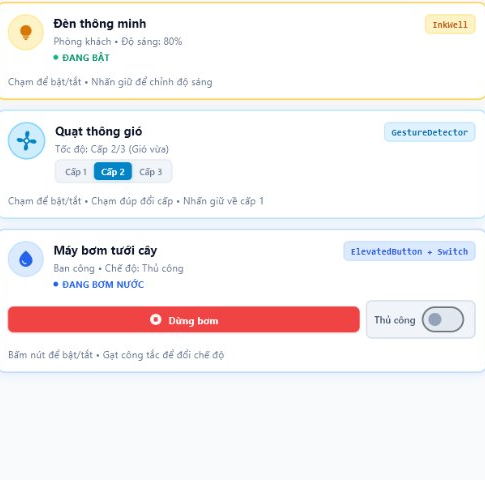
\includegraphics[width=\linewidth, height=5.50cm, keepaspectratio]{demo_devices_crop.png}%
      }
    \end{column}
    \hfill
    \begin{column}{0.48\textwidth}
      \centering
      {\footnotesize\bfseries\color{DarkMain} Nhật ký sự kiện thời gian thực (Event Log)}\\[0.08cm]
      \setlength{\fboxsep}{0pt}
      \fcolorbox{DarkMain!35}{white}{%
        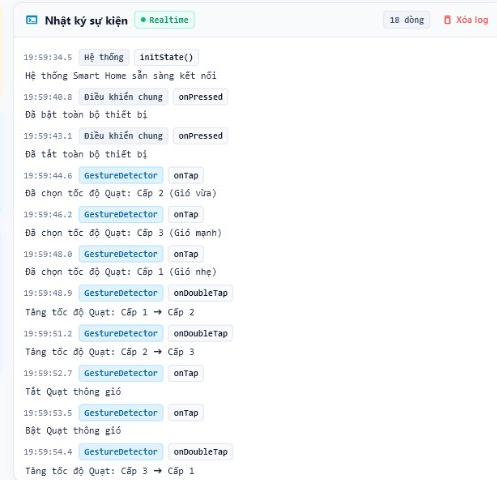
\includegraphics[width=\linewidth, height=5.50cm, keepaspectratio]{demo_log_crop.png}%
      }
    \end{column}
  \end{columns}
\end{frame}
\endgroup

% ------------------------------------------------------------------------------
% Slide 16: Luồng tương tác và xử lý dữ liệu
% ------------------------------------------------------------------------------
\begin{frame}{Luồng tương tác và xử lý dữ liệu}
  \vspace{0.18cm}
  \centering
  \begin{tikzpicture}
    \node[subbox, text width=2.35cm, minimum height=1.10cm, inner sep=2pt] (c1) at (-5.55, 0)
      {\textbf{Thẻ thiết bị}\\[1.5pt]{\scriptsize\color{TextMuted}Đèn, Quạt, Bơm}};
    \node[diagbox, text width=2.35cm, minimum height=1.10cm, inner sep=2pt] (c2) at (-1.85, 0)
      {\textbf{HomeScreen}\\[1.5pt]{\scriptsize\color{TextMuted}nhận Callback}};
    \node[subbox, text width=2.35cm, minimum height=1.10cm, inner sep=2pt] (c3) at (1.85, 0)
      {\textbf{Bộ nhớ RAM}\\[1.5pt]{\scriptsize\color{TextMuted}lưu dữ liệu logic}};
    \node[diagbox, text width=2.35cm, minimum height=1.10cm, inner sep=2pt] (c4) at (5.55, 0)
      {\textbf{Cập nhật UI}\\[1.5pt]{\scriptsize\color{TextMuted}vẽ lại \& ghi Log}};

    \draw[flowarrow] (c1.east) -- (c2.west) node[midway, above=3pt, font=\scriptsize\ttfamily\color{DarkMain}] {callback};
    \draw[flowarrow] (c2.east) -- (c3.west) node[midway, above=3pt, font=\scriptsize\ttfamily\color{DarkMain}] {update()};
    \draw[flowarrow] (c3.east) -- (c4.west) node[midway, above=3pt, font=\scriptsize\ttfamily\color{DarkMain}] {setState};
  \end{tikzpicture}

  \vspace{0.40cm}
  \begin{itemize}\setlength{\itemsep}{0.22cm}
    \item \textbf{Truyền ngược sự kiện}: thẻ con nhận cử chỉ rồi gọi \code{VoidCallback} báo lên màn hình cha
    \item \textbf{Tách \code{RamState} và biến \code{\_ui*}}: quan sát trực tiếp hiện tượng lệch dữ liệu giữa RAM và UI khi tắt \code{setState()}
    \item \textbf{Nhật ký thời gian thực}: ghi lại tên widget, loại callback và kết quả sau mỗi thao tác
  \end{itemize}
\end{frame}

% ------------------------------------------------------------------------------
% Slide 17: Trường hợp 1: Đèn thông minh (InkWell)
% ------------------------------------------------------------------------------
\begin{frame}[fragile]{Trường hợp 1: Điều khiển đèn bằng InkWell}
  \vspace{0.16cm}
  \begin{columns}[c, onlytextwidth]
    \begin{column}{0.49\textwidth}
      \begin{codepanel}
\begin{Verbatim}[commandchars=§«»,fontsize=\fontsize{7.1pt}{10.4pt}\selectfont]
Material(
  color: Colors.transparent,
  child: InkWell(
    borderRadius: BorderRadius.circular(16),
    onTap: widget.onTap,
    onLongPress: () {
      §cmt«// Báo cha ghi Log & mở bảng chỉnh độ sáng»
      widget.onLongPress();
      _showBrightnessModal(context);
    },
    child: ...,
  ),
)
\end{Verbatim}
      \end{codepanel}
    \end{column}
    \hfill
    \begin{column}{0.48\textwidth}
      \centering
      \setlength{\fboxsep}{0pt}
      \fcolorbox{DarkMain!35}{white}{%
        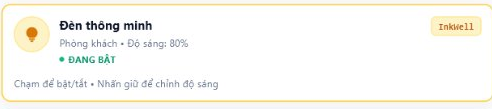
\includegraphics[width=\dimexpr\linewidth-0.8pt\relax]{demo_lamp_ui.png}%
      }

      \vspace{0.26cm}
      \raggedright
      \footnotesize
      \begin{itemize}\setlength{\itemsep}{0.18cm}
        \item \code{onTap}: gợn sóng Ripple, đèn đổi sang màu vàng, sáng viền thẻ
        \item \code{onLongPress}: mở bảng trượt \code{Slider} chỉnh độ sáng \textbf{10\% → 100\%}
      \end{itemize}
    \end{column}
  \end{columns}
\end{frame}

% ------------------------------------------------------------------------------
% Slide 18: Trường hợp 2: Quạt thông gió (GestureDetector)
% ------------------------------------------------------------------------------
\begin{frame}[fragile]{Trường hợp 2: Điều khiển quạt bằng GestureDetector}
  \vspace{0.16cm}
  \begin{columns}[c, onlytextwidth]
    \begin{column}{0.49\textwidth}
      \begin{codepanel}
\begin{Verbatim}[commandchars=§«»,fontsize=\fontsize{7.1pt}{10.4pt}\selectfont]
GestureDetector(
  behavior: HitTestBehavior.opaque,
  onTap: widget.onTap,             §cmt«// Bật / tắt»
  onDoubleTap: widget.onDoubleTap, §cmt«// Cấp 1->2->3»
  onLongPress: widget.onLongPress, §cmt«// Về cấp 1»
  child: ...,
)
\end{Verbatim}
      \end{codepanel}

      \vspace{0.18cm}
      {\footnotesize\color{TextMuted} \code{HitTestBehavior.opaque} giúp toàn bộ vùng trống trong thẻ đều bắt được cử chỉ chạm}
    \end{column}
    \hfill
    \begin{column}{0.48\textwidth}
      \centering
      \setlength{\fboxsep}{0pt}
      \fcolorbox{DarkMain!35}{white}{%
        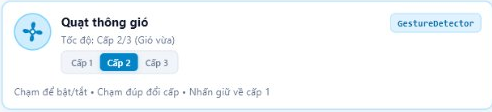
\includegraphics[width=\dimexpr\linewidth-0.8pt\relax]{demo_fan_ui.png}%
      }

      \vspace{0.24cm}
      \raggedright
      \footnotesize
      \begin{itemize}\setlength{\itemsep}{0.16cm}
        \item \code{onTap}: bật / dừng chuyển động xoay cánh quạt
        \item \code{onDoubleTap}: điều chỉnh tuần tự cấp tốc độ \textbf{1 → 2 → 3 → 1}
        \item \code{onLongPress}: đặt lại nhanh cấp gió về mức ban đầu (Cấp 1)
      \end{itemize}
    \end{column}
  \end{columns}
\end{frame}

% ------------------------------------------------------------------------------
% Slide 19: Điều khiển máy bơm và các nút điều khiển chung
% ------------------------------------------------------------------------------
\begin{frame}[fragile]{Trường hợp 3: Máy bơm và các nút điều khiển chung}
  \vspace{0.06cm}
  \begin{columns}[c, onlytextwidth]
    \begin{column}{0.49\textwidth}
      \begin{codepanel}
\begin{Verbatim}[commandchars=§«»,fontsize=\fontsize{7.1pt}{10.4pt}\selectfont]
§cmt«// 1. Máy bơm: nút bấm & công tắc chế độ»
ElevatedButton.icon(
  onPressed: widget.onTogglePower, ...
)
Switch(
  value: isAuto,
  onChanged: (bool val) =>
      widget.onToggleMode(val),
)

§cmt«// 2. Nút điều khiển chung: khóa khi đã tắt hết»
onPressed: hasAnyUiActive ? _turnOffAll : null,
\end{Verbatim}
      \end{codepanel}
    \end{column}
    \hfill
    \begin{column}{0.48\textwidth}
      \centering
      \setlength{\fboxsep}{0pt}
      \fcolorbox{DarkMain!35}{white}{%
        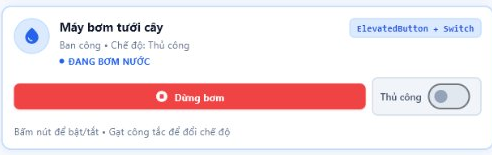
\includegraphics[width=\dimexpr\linewidth-0.8pt\relax]{demo_pump_ui.png}%
      }

      \vspace{0.06cm}
      \raggedright
      \footnotesize
      \begin{itemize}\setlength{\itemsep}{0.08cm}
        \item \code{onPressed}: đổi nhãn \textbf{Bật bơm} ↔ \textbf{Dừng bơm}, hiệu ứng nhấp nháy icon
        \item \code{Switch.onChanged}: nhận \code{bool val} (\code{ValueChanged<bool>}), đổi \textbf{Thủ công} ↔ \textbf{Tự động}
        \item Nút \textbf{Tắt tất cả} (điều khiển chung) tự vô hiệu hóa (\code{disabled}) khi mọi thiết bị đang tắt
      \end{itemize}
    \end{column}
  \end{columns}
\end{frame}

% ------------------------------------------------------------------------------
% Slide 20: Kiểm chứng vai trò setState()
% ------------------------------------------------------------------------------
\begin{frame}[fragile]{Trường hợp 4: Kiểm chứng vai trò setState()}
  \vspace{0.06cm}
  \begin{columns}[T, onlytextwidth]
    \begin{column}{0.50\textwidth}
      {\bfseries Các bước thử nghiệm}\\[0.10cm]
      \footnotesize
      \begin{enumerate}\setlength{\itemsep}{0.08cm}
        \item Gạt công tắc trên thanh công cụ sang \code{setState: Off}
        \item Thao tác bật Đèn, đổi cấp Quạt $\to$ quan sát biến trong RAM
        \item Gạt lại \code{setState: On} $\to$ giao diện được cập nhật đồng bộ
      \end{enumerate}

      \vspace{0.10cm}
      \begin{codepanel}
\begin{Verbatim}[commandchars=§«»,fontsize=\fontsize{7.8pt}{11pt}\selectfont]
_ramController.updateLamp(isOn: newOn);
if (!_simulateForgetSetState) {
  setState(() => _syncUiFromRam());
}
\end{Verbatim}
      \end{codepanel}
    \end{column}
    \hfill
    \begin{column}{0.47\textwidth}
      \centering
      \setlength{\fboxsep}{0pt}
      \fcolorbox{DarkMain!35}{white}{%
        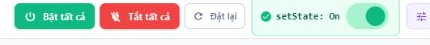
\includegraphics[width=\dimexpr\linewidth-0.8pt\relax]{demo_state_header.png}%
      }

      \vspace{0.18cm}
      \renewcommand{\arraystretch}{1.20}
      \setlength{\tabcolsep}{4.5pt}
      \footnotesize
      \begin{tabular}{@{} l l l @{}}
        \toprule[0.8pt]
        {\bfseries\color{DarkMain}Chế độ} & {\bfseries\color{DarkMain}RAM} & {\bfseries\color{DarkMain}Giao diện} \\
        \midrule[0.45pt]
        \code{setState: Off} & Đã cập nhật & \textbf{Không đổi} \\
        \code{setState: On}  & Đã cập nhật & \textbf{Đồng bộ ngay} \\
        \bottomrule[0.8pt]
      \end{tabular}

      \vspace{0.16cm}
      \begin{tcolorbox}[colback=CodeBg, colframe=DarkMain, left=6pt, right=6pt, top=4pt, bottom=4pt]
        {\scriptsize\bfseries Minh chứng lệch dữ liệu khi tắt \code{setState()}:}\\[2pt]
        {\fontsize{7.3pt}{9.6pt}\selectfont\raggedright
        $\bullet$ \textbf{Tắt setState}: Nhấn Đèn $\to$ RAM cập nhật bật, nhưng thẻ Đèn \textbf{vẫn TẮT}.\\[1.5pt]
        $\bullet$ \textbf{Bật lại setState}: Framework dựng lại $\to$ Đèn \textbf{sáng ngay lập tức} không cần bấm lại.
        }
      \end{tcolorbox}
    \end{column}
  \end{columns}
\end{frame}

% ==============================================================================
% PHẦN 4: TÀI LIỆU THAM KHẢO & KẾT THÚC
% ==============================================================================

% ------------------------------------------------------------------------------
% Slide 21: Tổng kết và bài học kinh nghiệm
% ------------------------------------------------------------------------------
\setsectionfooter{Tổng kết}
\begin{frame}{Tổng kết và bài học kinh nghiệm}
  \vspace{0.08cm}
  \begin{columns}[T, onlytextwidth]
    \begin{column}{0.48\textwidth}
      \begin{codepanel}
        {\bfseries\color{DarkMain} 1. Tiếp nhận sự kiện qua Callback}\\[3pt]
        {\small\raggedright
        Dùng \code{VoidCallback} và \code{ValueChanged<T>} chuyển tiếp tương tác từ widget con lên widget cha.
        }
      \end{codepanel}

      \vspace{0.08cm}
      \begin{codepanel}
        {\bfseries\color{DarkMain} 2. Lưu giữ trạng thái trong lớp State}\\[3pt]
        {\small\raggedright
        Biến trạng thái phải nằm trong lớp \code{State} (bộ nhớ RAM), tuyệt đối không đặt cục bộ trong \code{build()}.
        }
      \end{codepanel}
    \end{column}
    \hfill
    \begin{column}{0.48\textwidth}
      \begin{codepanel}
        {\bfseries\color{DarkMain} 3. Đồng bộ giao diện bằng setState()}\\[3pt]
        {\small\raggedright
        Báo cho \code{framework} lên lịch dựng lại ở frame kế tiếp; quên gọi sẽ gây lệch trạng thái giữa RAM và UI.
        }
      \end{codepanel}

      \vspace{0.08cm}
      \begin{codepanel}
        {\bfseries\color{DarkMain} 4. Lưu ý thực tế khi mở rộng app}\\[3pt]
        {\small\raggedright
        Kiểm tra \code{if (!mounted) return;} sau tác vụ \code{async}; ưu tiên dùng Provider khi ứng dụng lớn hơn.
        }
      \end{codepanel}
    \end{column}
  \end{columns}
\end{frame}

% ------------------------------------------------------------------------------
% Slide 22: Tài liệu tham khảo
% ------------------------------------------------------------------------------
\setsectionfooter{Tài liệu tham khảo}
\begin{frame}{Tài liệu tham khảo}
  \vspace{0.02cm}
  \begin{enumerate}\setlength{\itemsep}{0.10cm}
    \footnotesize
    \item Flutter Documentation, \textit{`Handling gestures''}, Google.\\
          {\color{DarkMain}\url{https://docs.flutter.dev/ui/interactivity/gestures}}
    \item Flutter Documentation, \textit{`Adding interactivity to your Flutter app''}, Google.\\
          {\color{DarkMain}\url{https://docs.flutter.dev/ui/interactivity}}
    \item Flutter Documentation, \textit{`Differentiate between ephemeral state and app state''}, Google.\\
          {\color{DarkMain}\url{https://docs.flutter.dev/data-and-backend/state-mgmt/ephemeral-vs-app}}
    \item Dart Documentation, \textit{`Functions''}, Google.\\
          {\color{DarkMain}\url{https://dart.dev/language/functions}}
    \item TS. Nguyễn Duy Nhật Viễn, \textit{`Bài giảng Lập trình Đa nền tảng''}, Khoa Điện tử và Trí tuệ Nhân tạo, Trường Đại học Bách khoa -- Đại học Đà Nẵng, 2026.
  \end{enumerate}

  \vspace{0.14cm}
  \begin{codepanel}
    {\footnotesize\bfseries\color{TextDark} Mã nguồn chương trình thực nghiệm trên GitHub}\\[1.5pt]
    {\footnotesize\color{DarkMain}\url{https://github.com/KhoaLe246205/cross-platform/tree/main/event_interaction}}
  \end{codepanel}
\end{frame}

% ------------------------------------------------------------------------------
% Slide 23: Kết thúc
% ==============================================================================
\setsectionfooter{}
\begin{frame}
  \vspace{1.95cm}
  \centering
  {\fontsize{19.5pt}{25pt}\selectfont\bfseries\color{DarkMain}
    Cảm ơn Thầy và các bạn đã lắng nghe!\par
  }
\end{frame}

\end{document}
